\documentclass[12pt, french]{article}

\usepackage{fancyhdr, fancybox, lastpage,mhchem}
\usepackage[most]{tcolorbox}
\usepackage[a4paper, margin={0.3in, .75in}]{geometry}
\usepackage{wrapfig}
\pagestyle{fancy}
\renewcommand\headrulewidth{1pt}
\renewcommand\footrulewidth{1pt}
\fancyhf{}
\rhead{ \em{Zakaria Haouzan}}
\lhead[C]{\em{2ème année baccalauréat Sciences Physiques}}
\chead[C]{}
\rfoot[C]{}
\lfoot[R]{}
\cfoot[]{\em{Page \thepage / \pageref{LastPage}}}


\newtcolorbox{Box2}[2][]{
                lower separated=false,
                colback=white,
colframe=white!20!black,fonttitle=\bfseries,
colbacktitle=white!30!gray,
coltitle=black,
enhanced,
attach boxed title to top left={yshift=-0.1in,xshift=0.15in},
title=#2,#1}


\begin{document}
\begin{center}
   \shadowbox {\bf{Les transformations liée a
des réactions acides et bases
}
 }

\end{center}

\vspace{-0.2cm}
%%_________________________Exercice ! :"_________________________Exercice
   \begin{Box2}{Exercice 1 : Ibuprofène  \dotfill{400mg}}

\begin{wrapfigure}{r}{0.22\textwidth}
  \begin{center}
	  \vspace{-0.6cm}
	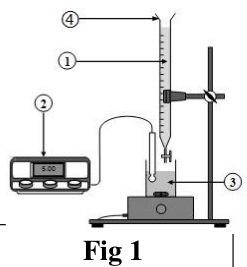
\includegraphics[width=0.22\textwidth]{./img/Dosage_00.png}
	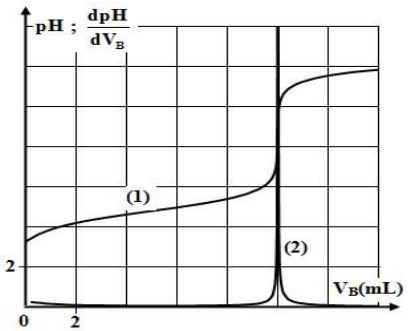
\includegraphics[width=0.22\textwidth]{./img/Dosage_00_1.png}
  \end{center}
\end{wrapfigure}


L’étiquette d’un médicament fournit l'information "Ibuprofène…. 400 mg ".
On dissout un comprimé contenant l’ibuprofène selon un protocole bien défini afin
d'obtenir une solution aqueuse (S) d’ibuprofène de volume $V_S =100 mL$ .
Pour vérifier, la masse d’ibuprofène contenu dans ce comprimé, on procède à un titrage acido-basique du volume $V_S$ par une solution aqueuse d’hydroxyde de sodium $(Na^+_{(aq)}  + HO^-_{(aq)})$ de concentration molaire $C_B = 1,94.10^{-1} mol.L^{-1}$ , en utilisant le dispositif
expérimental de la figure (1).

La figure (2) donne les courbes $pH=f(V_B)$ et $\frac{dpH}{dV_B} = g(V_B)$ obtenues lors de ce dosage.

1. Nommer les éléments du dispositif expérimental numérotés 1,2 ,3 et 4
sur la figure (1).

2. Parmi les courbes (1) et (2) de la figure (2), quelle est celle qui
représente pH = f (VB) ?

3. Déterminer graphiquement la valeur du volume $V_{BE}$, versé à
l'équivalence.

4. Écrire l’équation de la réaction qui a eu lieu lors du dosage sachant
qu'elle est totale.

5. Calculer la valeur de la quantité de matière nA d'ibuprofène dans la
solution(S).

6. Déduire la valeur de la masse m d’ibuprofène dans le comprimé et la
comparer à celle indiquée sur l'étiquette du médicament.

   \end{Box2}


%%_________________________Exercice !2 :"_________________________Exercice
\begin{Box2}{Exercice 2 : Dosage acide-base d’une
solution diluée d’ammoniac.}
\begin{wrapfigure}{r}{0.47\textwidth}
  \begin{center}
	  \vspace{-0.6cm}
	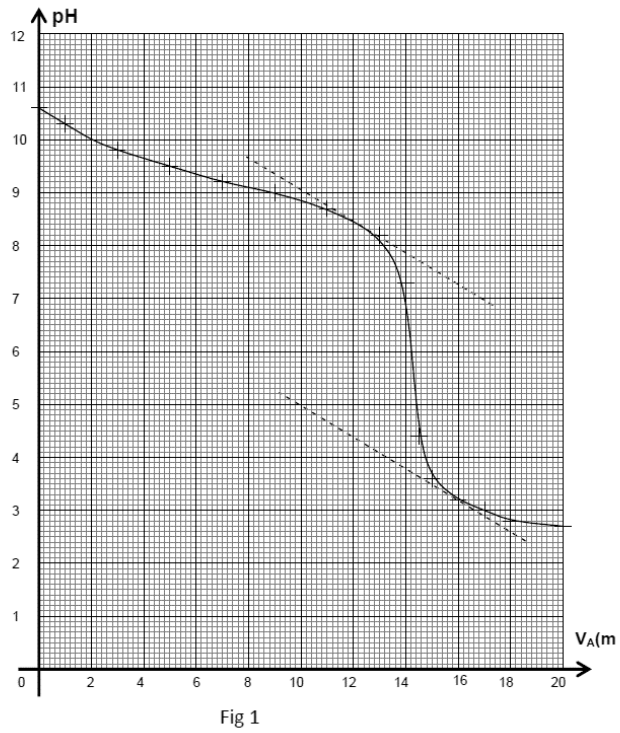
\includegraphics[width=0.47\textwidth]{./img/Dosage_01_00.png}
  \end{center}
\end{wrapfigure}
Pour déterminer la concentration $C_B$ d’une solution
commerciale concentrée d’ammoniac, on procède
par dosage acido-basique. On prépare par dilution une solution S de concentration $C' = \frac{C_B}{1000}$.

On réalise le dosage pH métrique d’un volume $V $=$20 mL$ de la solution S à l’aide d’une solution $S_A$ d’acide chlorhydrique $(H_3O^+_{(aq)} + Cl^-_{(aq)}$ de concentration $C_A = 0,015mol.L^{-1}$.

On mesure le pH du mélange après chaque addition
d’un volume d’acide ; Les résultats obtenus
permettent de tracer la courbe de dosage $pH = f(V_A)$
(fig 1). On atteint l’équivalence lorsqu’on ajoute du
dosage.

1. En utilisant la valeur du pH correspondant à
l’addition de 5mL d’acide chlorhydrique,
calculer le taux d’avancement final de la
réaction du dosage. Conclure.

2. Déterminer le volume $V_{AE}$ En déduire $C'$et $C_B$.

3. Parmi les indicateurs colorés indiqués dans le tableau ci-
dessous, choisir celui qui conviendra le mieux à ce dosage.

\begin{center}
\begin{tabular}{ |c||c|c|c| } 
 \hline
 L'indicateur coloré & phénolphtaléine& Hélianthine &Rouge de Chlorophénol  \\\hline 
 Zone de virage		 & 8,2 - 10		   &  5,2 - 6,8 & 3,1- 4,4 \\  
 \hline
\end{tabular}
\end{center}

\end{Box2}

%%_________________________Exercice ! 3:"_________________________Exercice
\begin{Box2}{Exercice 3 :Étude d’un système chimique à l’état d’équilibre }


	\textbf{1. }On considère une solution aqueuse $(S_0)$ d’ammoniac $NH_3$, de volume $V_0$ et de concentration molaire $C_0 = 1,0 . 10^{-2}mol/L$ . Le pH de cette solution à 25°C vaut pH = 10,6.

	1.1. Écrire l’équation de la réaction modélisant la transformation entre l’ammoniac et l’eau.

	1.2. Construire le tableau d’avancement.

	1.3. Calculer le taux d’avancement de cette réaction.

	1.4. Calculer la concentration molaire effective des ions ammonium $NH^+_4$ à l’etat d’équilibre du système.

	1.5. Calculer la constante d’équilibre K et déduire la valeur de pKA la constate d’acidité du couple $NH^+/NH_3$.
	
	1.6. On mélange un volume de la solution $(S_0)$ d’ammonium avec un volume d’une solution de chlorure d’ammonium $(NH_{4(aq)}^+ + Cl^-_{(aq)})$. le pH du mélange est pH = 6,2. Tracer le diagramme de prédominance du couple    $NH^+_4/NH_3$ . En déduire l’espèce prédominante de ce couple dans le mélange.

	\textbf{2- Dosage d’un engrais : \dotfill}

Le nitrate d’ammonium $NH_4NO_3$ est un composée ionique présent dans divers engrais. Un sac d’engrais porte
l’indication suivantes : \textbf{" pourcentage en masse 75\% de nitrate d’ammonium ".}

Pour vérifier le pourcentage massique en nitrate d’ammonium indiqué par le producteur, on prépare une solution
aqueuse $(S_A)$ par dissolution de la masse $m=15,0g$ d’engrais dans le volume $V_0 = 1L$ d’eau distillée. On dose les ions
ammonium $NH_4^+$ présent dans un volume $V_A = 10,0 mL$ de la solution $(S_A)$ par une solution aqueuse $(S_B)$ d’hydroxyde de sodium $ (Na^+_{(aq)} +  HO^-_{(aq)})$ de concentration molaire $C_B = 0,10 mol.L-1$. Le volume de la solution $(S_B)$ versé à l’équivalence est $V_{BE} = 14,0mL$.

\textbf{Donnée :$M(NH_4NO_3) = 80 g/mol$ et $K_e = 10^{-14}$}

2.1. Écrire l’équation de la réaction qui se produit au cours du dosage.

2.2. Déterminer la valeur de la concentration molaire $C_A$ des ions ammonium $NH_4^+$ dans la solution $(S_A)$.

2.3. Calculer le pourcentage massique en masse de nitrate d’ammonium contenu dans cet engrais. Comparer à la valeur annoncée par le fabriquant

2.4. Déterminer l’indicateur colorée convenable a ce dosage

\textbf{3- Dosage de la solution $(S_b)$ d’ammoniac :\dotfill}
\begin{wrapfigure}{r}{0.37\textwidth}
  \begin{center}
	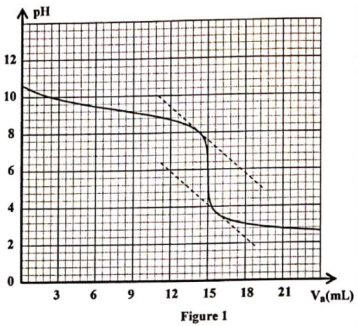
\includegraphics[width=0.37\textwidth]{./img/Dosage_02.png}
  \end{center}
\end{wrapfigure}
On prépare une solution $(S_B)$ de volume $V$, en diluant $100$ fois une solution commerciale d’ammoniac $S_0$ de concentration $C_0$.

On réalise un dosage pH-métrique d’un volume Vb = 15 mL de la solution $S_B$ par une solution aqueuse $S_a$ d’acide chloridrique $(H_3O^+_{(aq)} + Cl^-_{(aq)})$ de concentration $C_a = 10^{-2} mol/L$ . La courbe de la figure 1 représente
les variations du pH du mélange en fonction du volume Va versée de la
solution $S_b$ : $pH = f(V_a)$.

3.1. Écrire l’équation de la réaction de dosage.

3.2. Calculer K la constate d’équilibre associée à la réaction

3.3. Calculer la concentration $C_b$ de la solution $S_b$. En déduire $C_0$.

3.4. Choisir en justifiant, parmi les indicateurs colorés suivants, l’indicateur adéquat pour réaliser ce dosage.
\begin{center}
\begin{tabular}{ |c||c|c|c| } 
 \hline
 L'indicateur coloré & phénolphtaléine& Hélianthine &Rouge de Chlorophénol  \\\hline 
 Zone de virage		 & 8,2 - 10		   &  5,2 - 6,8 & 3,1- 4,4 \\  
 \hline
\end{tabular}
\end{center}


3.5.Calculer le taux d’avancement final, de la réaction de dosage lorsque le volume de la solution versé est  $S_a$ est $V_a = 9mL$.


\end{Box2}

%%_________________________Exercice 4 : _________________________Exercice
\begin{Box2}{Exercice 4 : Vérification du degré d’acidité du vinaigre commercial }
   % \begin{wrapfigure}[12]{r}{0.5\textwidth}
  %\begin{center}
	  %\vspace{-0.6cm}
	%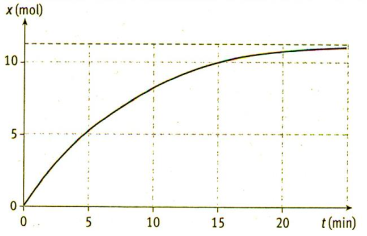
\includegraphics[width=0.5\textwidth]{./img/ex4.png}
  %\end{center}
%\end{wrapfigure}
\emph{Le vinaigre est une solution aqueuse d’acide éthanoïque $(CH_3COOH)$, il est
caractérisé par son degré d’acidité (X°) qui représente la masse (en gramme)
d’acide éthanoïque contenue dans 100 g de solution.}

\textbf{Données :}

\begin{itemize}

	\item Toutes les mesures ont été faites à 25°C.
	\item La masse volumique du vinaigre : $\rho = 1 g/mL$.
	\item La masse molaire de l’acide éthanoïque : $M(CH_3COOH) = 60 g/mol$.
	\item La conductivité molaire ionique de l’ion $H_3O^+ $.

\end{itemize}
On extrait un échantillon de vinaigre commetcial, de volume $V_0 = 1 mL$, de
concentration molaire $C_0$ et portant l’indication (7°), on y ajoute de l’eau distillée
pour préparer une solution (S) de concentration molaire $C_S$ et de volume $V_S = 100 mL$.

On neutralise un échantillon de volume $V_A= 20 mL$ de la solution (S) à l’aide d’une
solution aqueuse $(S_B)$ d’hydroxyde de sodium $(Na^+_{(aq)} + OH^-_{(aq)})$ de concentration molaire $C_B = 1,5.10^{-2} mol/L$.

L’équivalence est obtenue lorsque le volume vérsé de la solution $(S_B)$ est : $V_{BE} = 15,7 mL$.

1. Ecrire l’équation modélisant la réaction ayant lieu au cours du dosage.

2. Calculer la valeur de $C_S$.

3. Déterminer le degré d’acidité du vinaigre étudié. Le résultat obtenu est-il en accord avec l’indication inscrite sur le vinaigre commercial ou non ?

\end{Box2}

\vspace{-0.8cm}
\begin{center}
   \Large{ \em{Exercices Supplémentaires}}
\end{center}


\vspace{-0.6cm}
%%_________________________Exercice 5 : _________________________Exercice
\begin{Box2}{Exercice 5 : }
	\begin{wrapfigure}[14]{r}{0.5\textwidth}
  \begin{center}
	  \vspace{-0.6cm}
	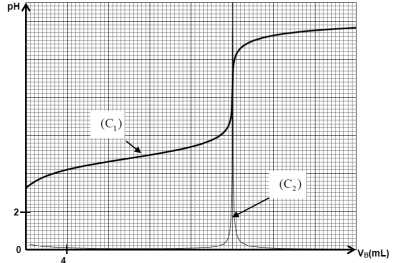
\includegraphics[width=0.5\textwidth]{./img/Dosage_03.png}
  \end{center}
\end{wrapfigure}
On prépare une solution aqueuse
(SA) d’acide éthanoïque $CH_3COOH$ de
volume $V = 1L$ et de concentration
molaire $C_A$, en dissolvant une quantité
de masse $m$ de cet acide dans l’eau distillée.

On dose un volume $V_A = 20mL$ de
la solution $(S_A)$ en suivant les
variations du pH en fonction du
volume VB versé d’une solution
aqueuse d’hydroxyde de sodium $(Na^+_{(aq)} +  HO^-_{(aq)})$ de concentration molaire $C_B = 2.10^{-2}mol/L$.

1. Ecrire l’équation chimique modélisant la réaction du dosage.

2. A partir des mesures obtenues, on a tracé la courbe $(C_1)$ représentant $pH = f(V_B)$ et la courbe $(C_2)$.représentant $\frac{dpH}{dV_B} = g(V_B)$

2.1. Déterminer le volume $V_{BE}$ de la solution d’hydroxyde de sodium versé à l’équivalence.

2.2. Trouver la valeur de la masse m nécessaire à la préparation de la solution $(S_A)$.

2.3. Montrer que la réaction entre l’acide éthanoïque et l’eau est limitée.

\end{Box2}


%\begin{Box2}{Exercice 6 : }
	

%\end{Box2}


%\begin{Box2}{Exercice 7 : }


%\end{Box2}


%\begin{Box2}{Exercice 8 : }



%\end{Box2}
\end{document}
